\documentclass[11pt]{article}
\usepackage{amsmath, amssymb, amsthm, bm}
\usepackage[margin=2.4cm]{geometry}
\usepackage{booktabs, graphicx, float, caption}
\usepackage{xeCJK}
\setCJKmainfont{Noto Serif CJK SC}
\setCJKsansfont{Noto Sans CJK SC}
\usepackage{titlesec}
\titleformat{\section}{\centering\Large\bfseries}{\thesection}{1em}{}
\newtheorem{assumption}{假设}
\newtheorem{proposition}{命题}
\newtheorem{definition}{定义}
\captionsetup{font=small}
\renewcommand{\figurename}{图}
\renewcommand{\tablename}{表}
\renewcommand{\abstractname}{摘\quad 要}
\renewcommand{\refname}{参考文献}
\renewcommand{\appendixname}{附录}
\setlength{\parskip}{2pt plus 1pt}
\linespread{1.12}

\title{\textbf{算力约束下提升大语言模型能力的资源配置建模\\[4pt]
\large ——问题一、二：数据质量评价、领域配比与广义标度律}}
\author{}
\date{2026 年 9 月 23 日}

\begin{document}
\maketitle

\begin{abstract}
\noindent 本文研究预训练语料的质量评价、领域配比及其与模型规模的联合作用规律。
\textbf{问题一}：对 27.2 万篇文档的 22 个异质质量信号，建立"定向标量化—域内稳健归一—CRITIC 客观赋权—加权几何平均"的评分管线，得到样本级与域级连续质量分 $Q$；以四组信号的域内分位排名极差定义指标冲突，用冲突率—阈值曲线自适应确定阈值 $\tau=0.75$，测得冲突率 $21.5\%$ 并在两个全量扩展集上复现，采用 Huber 连续降权消解；对 512 组小模型配比实验做中心对数比（clr）变换后回归，检验集 $R^2$ 由裸回归的 $0.654$ 提升至 $0.772$，进而给出 $17\times13$ 领域迁移矩阵与最优配比 $\bm p^*$（相对均匀配比预测降损 $9.9\%$，95\% CI $[9.7\%,14.1\%]$）。域级质量分与训练边际价值的秩相关仅 $-0.06$，定量证实"内在质量不等于训练价值"。
\textbf{问题二}：数据审计发现 B1 为公式生成锚点，B6/B7 可由线性乘性耦合以噪声水平刻画。嵌套族交叉验证选出主模型（cv-RMSE $0.0497$），广义标度律为 $L=\{E+AN^{-\alpha}[1+\kappa_N(1-Q)]+BD^{-\beta}[1+\kappa_D(1-Q)]+k_0(1-Q)\}\cdot e^{s(N)[\bar f(\bm p)-\bar f(\bm p^*)]}$，主口径 $Q_{\mathrm B}=\bar q(\bm p)$、$Q_0=0.6609$。闭式结果与数值解互验。主要结论：在 $(10^{10},10^{12},0.9)$ 处质量弹性约为参数弹性的 $3.7$ 倍；质量从 $0.5$ 提到 $0.6$，在算力最优点等效于参数扩大 $1.29$--$1.77$ 倍（$C=10^{20}$--$10^{24}$）；低质量造成规模不可弥补的损失下界 $(1-Q)k_0$（半合成数据内建）；数据质量越高，算力最优配置越偏向"小模型、多数据"。

\vspace{4pt}
\noindent\textbf{关键词}：数据质量评价；指标冲突；成分数据回归；广义标度律；算力最优配置
\end{abstract}

\section{问题重述}

\subsection{问题背景}

大语言模型能力的提升依赖参数规模 $N$、训练数据量 $D$、数据质量 $Q$ 与领域配比 $\bm p$ 的协同配置，而算力预算约束使四者之间存在权衡。工业实践（FineWeb-Edu、DCLM、RegMix 等）表明：数据侧工程能以远低于扩大规模的成本换取同等能力增益，但"质量"缺乏可进入数学模型的连续度量，配比决策也长期依赖人工经验。赛题提供三组附件：A（质量信号与配比实验）、B（标度律观测）、C（能力评测），要求以可核验的建模回答资源配置问题。

\subsection{问题描述}

\textbf{问题一}：基于附件 A 的 22 个质量指标，(a) 建立样本级与域级综合质量评分；(b) 定义并消解指标间冲突，在扩展集上复验；(c) 建立 17 域训练配比与 13 个验证域交叉熵损失的定量关系，用三种规模的留出实验验证，并讨论向 10B/70B 外推的稳健性。

\textbf{问题二}：融合附件 B 的多来源数据，将问题一输出的质量分 $Q$ 与配比 $\bm p$ 引入经典标度律 $L=E+AN^{-\alpha}+BD^{-\beta}$，建立广义损失律；给出各因素的弹性与相互替代关系（如"质量提高 0.1 等效于增加多少参数"）。

\textbf{问题三、四}（后续报告）：算力预算约束下的资源配置优化与结构性转移识别；能力增长的规模/非规模因素分解与前沿预测。

\section{问题分析}

\subsection{总体思路}

四问构成递进链：问题一把数据侧压缩为两个可注入的量——连续质量分 $Q$ 与配比—损失关系 $f(\bm p)$；问题二将其嵌入标度律得到 $L(N,D,Q,\bm p)$；问题三在成本约束下优化该损失；问题四将损失翻译为能力得分。因此问题一的每项产出都须落盘为明确接口（表~\ref{tab:iface}），问题二的自变量口径须与问题一逐字一致。

数据处理遵循\textbf{证据分层}原则：直接观测（A1--A11）优先支撑主结论；半合成与插值数据（B2、B6--B8）用于形式选择并明示假设；外推生成数据（A12--A15、B10）只作稳健性讨论，不充当验证。建模顺序为：数据审计 $\to$ 质量评分与冲突消解 $\to$ 配比回归与跨尺度验证 $\to$ 标度律形式选择与拟合 $\to$ 解析理论与互验。

\subsection{各问题的关键难点}

\textbf{问题一的难点}：其一，22 个指标形态异质（8 个 logits 列表字段、3 个负对数比、15 个规则统计量），方向与量纲不一，且 github/arxiv 等域的指标基线存在结构性差异，直接聚合会把域间差异误判为质量差异；其二，冲突若用预设阈值定义会陷入"定义决定结论"的循环论证；其三，配比是成分数据（$\sum_ip_i=1$），直接回归产生闭合效应伪相关；其四，17 个配比域中仅 6 个有官方质量映射，其余 11 个域需自建关联。

\textbf{问题二的难点}：其一，附件 B 各表来源与噪声水平差异极大，须先审计再拟合，避免把不同源数据拼成同一因变量；其二，质量进入损失的函数形式（加性惩罚 vs 有效数据乘子）不能先验指定，须由数据选择；其三，附件 B 的 $Q$ 与问题一的 $Q$ 同范围不同尺度，须建立口径换算并作为显式假设。

\section{模型假设}

\begin{assumption}[质量信号可信]\label{asm:signal}
附件 A 的 22 个质量信号按其原始定义（Meta-rater 信号体系）如实计算，logits 字段经 softmax 后的概率/期望具有序数意义。适用条件：仅用于文档间相对比较，不解释为绝对语言学度量。
\end{assumption}

\begin{assumption}[小代理可迁移]\label{asm:proxy}
配比对各验证域损失的\emph{排序}效应在 1M--1B 参数范围内近似保持。本假设不作先验接受，由三尺度留出集实证检验（\S\ref{sec:m1c}），检验结果决定其适用边界。
\end{assumption}

\begin{assumption}[质量口径锚定]\label{asm:anchor}
主口径取“完美教材 $\Leftrightarrow$ 经典式”：$Q_{\mathrm B}=\bar q(\bm p)$，基线质量 $Q_0=\bar q(\bm p^*)=0.6609$。副口径取“当前推荐配比语料 $\Leftrightarrow$ 经典式”：$Q_{\mathrm B}=\bar q(\bm p)/0.6609$。早期 Pile 锚点 $Q_{\mathrm{ref}}=0.5608$ 已废弃，因为 B1 与 Hoffmann 等（2022）的常数吻合到 $\mathrm{RMSE}=1.6\times10^{-4}$，是公式生成数据。
\end{assumption}

\begin{assumption}[评价权重固定]\label{asm:weight}
汇总 13 个验证域损失的评价权重 $\bm w$ 取等权（主口径）并全文唯一；$\bm w$ 与被优化的配比 $\bm p$ 严格分离，避免"改考卷"与"改备考策略"混淆。pile\_cc 单域口径作为副口径报告。
\end{assumption}

\begin{assumption}[成本代理有效]\label{asm:cost}
问题二仅使用 $C\approx6ND$ 作为训练算力代理（用于最优配置推导）；质量成本与注意力成本留待问题三引入。
\end{assumption}

\section{符号说明}

\begin{table}[H]
\centering\small
\caption{主要符号及含义}
\begin{tabular}{clc}
\toprule
符号 & 含义 & 单位/范围 \\
\midrule
$N,\,D$ & 模型参数量、训练 token 数 & 个（代入公式用实际值） \\
$Q,\;Q_{\mathrm B}$ & 综合质量分（问题一口径）、B 口径质量 & $[0,1]$；主口径 $Q_{\mathrm B}=\bar q$ \\
$\bm z_i,\;Q(x_i)$ & 文档 $i$ 的 25 维标准化指标、样本级质量分 & $[0,1]$ \\
$\bar Q_d$ & 域 $d$ 的域级质量分（中位数主口径） & $[0,1]$ \\
$c(x),\;\tau$ & 文档冲突度、自适应冲突阈值 & $[0,1]$ \\
$\bm p\in\Delta^{16}$ & 17 域训练配比，$p_i\ge0,\ \sum_ip_i=1$ & 单纯形 \\
$\bm z=\mathrm{clr}(\bm p)$ & 配比的中心对数比坐标 & $\mathbb R^{17},\ \sum z_i=0$ \\
$L_v,\;L_{\mathrm{tgt}}$ & 验证域 $v$ 的交叉熵、按 $\bm w$ 加权的目标损失 & nats \\
$T_{iv}$ & 迁移矩阵：$\partial\ln L_v/\partial p_i$（均匀配比处） & --- \\
$\nu_d$ & 域 $d$ 的训练边际价值 & --- \\
$E,A,\alpha,B,\beta$ & 标度律基线参数 & 见表~\ref{tab:params} \\
$k_0,\,\kappa_N,\,\kappa_D$ & 质量地板系数、质量对参数项与数据项的耦合强度 & nats，无量纲 \\
$h_N,\,h_D,\,s(N)$ & $1+\kappa(1-Q)$；配比强度 $1.003-0.077\log_{10}(N/10^6)$ & 无量纲 \\
$\varepsilon_N,\varepsilon_D,\varepsilon_Q$ & 损失对各因素的弹性 & --- \\
$C$ & 训练算力预算（$C\approx6ND$） & FLOPs \\
\bottomrule
\end{tabular}
\end{table}

仅列全文反复使用的符号，局部符号在首次出现处说明。

\section{模型的建立与求解}

\subsection{数据预处理与审计}\label{sec:prep}

\textbf{数据审计发现（先于一切建模）}。逐表核对附件实际文件得到四个影响建模路线的事实：(i) A10/A11（1B 验证集）配比表 64 行、损失表 63 行，按 \texttt{index} 取交集使用；(ii) A16 的 17 域映射中仅 3 个 direct、3 个 near\_direct，11 个域无质量映射（inferred）；(iii) B1（Pythia 训练日志 1{,}176 行）可被三参数形式拟合至 $\mathrm{RMSE}=1.5\times10^{-4}$，呈公式生成特征；(iv) B8 与 B6/B7 在相同 $(N,D,Q)$ 点损失相关 $-0.03$ 且方向相反，两表不可比，B8 不参与联合拟合。

\textbf{指标展开}。22 个字段按输出形态展开为 25 个指标：二元 logits（\texttt{fluency\_en}、\texttt{ad\_en}）取 $\mathrm{softmax}$ 后正类概率；6 档 logits（\texttt{modernbert} 四字段）取期望档位 $\sum_k k\,\sigma_k/5$；\texttt{qurater} 拆为写作/专业/事实/教育四个独立维度；\texttt{fineweb\_edu} 直取；DSIR 三项为负对数比，仅域内可比；15 个规则统计量按定义方向处理。

\textbf{域内稳健归一}。每域每指标依次做：适宜区间型指标（词数、词长、一元熵等）以距域内中位数偏离改单峰；重尾指标先 $\log(1+x)$；$1\%/99\%$ 缩尾；域内 Min--Max 至 $[0,1]$；负向指标取补。全部变换参数在 A1 上估计后\textbf{冻结}，原样应用于 A2/A3——否则管线差异会混入抽样偏差，破坏对照的归因（这也是"同一管线"为题目强制的原因）。A1--A3 缺失率均低于 $0.03\%$，以域内中位数填补。

\subsection{问题一 (a)：综合质量评分}\label{sec:m1a}

\textbf{主线：CRITIC 客观赋权 + 加权几何平均。}指标 $j$ 的信息量与权重为
\begin{equation}
C_j=\sigma_j\sum_{k=1}^{25}\bigl(1-r_{jk}\bigr),\qquad
w_j=C_j\Big/\sum_k C_k,\qquad
Q(x)=\prod_{j=1}^{25} z_j(x)^{\,w_j},
\label{eq:critic}
\end{equation}
其中 $\sigma_j$ 为对比强度、$r_{jk}$ 为指标相关。选 CRITIC 而非熵权，是因其额外惩罚冗余指标（如 \texttt{fluency} 与 \texttt{readability} 高相关时权重自动分摊）；选几何平均而非算术平均，是因乘法形式实现"短板支配"——广告概率经补转换趋零时总分被显著压低，与 FineWeb-Edu/DCLM 的一票否决式过滤实践的方向一致但保留连续性。

\textbf{对照方法组}。等权几何平均、PCA（取累计方差 $80.6\%$ 的 10 个主成分、按方差贡献率合成，载荷矩阵输出至附表）、TOPSIS（以 CRITIC 权重加权的理想解贴近度）、K-means 三档聚类（仅给"优/普通/劣"相对档位）。样本级排序一致性：CRITIC 对等权 Spearman $0.991$、对 TOPSIS $0.946$、对 PCA $0.871$——三套互不蕴含的赋权假设给出高度一致的排序，说明质量结构是数据内在的而非赋权人为制造；K-means 的档位边界与连续分的分位一致，但聚类无法输出问题三成本函数所需的连续 $Q$，故仅作佐证。

\textbf{域级聚合与抽样代表性}。域级分取中位数主口径并报 token 加权副口径与 bootstrap 95\% CI（$B{=}2000$）。七域排序：arxiv $0.713>$ stackexchange $0.590>$ commoncrawl $0.557>$ github $0.533>$ book $0.511>$ c4 $0.499>$ wikipedia $0.484$（图~\ref{fig:box}）。以同一冻结管线复算 A2（arxiv 全量 17{,}523 篇）与 A3（github 全量 203{,}752 篇）：与 A1 对应子集的 KS 检验 $D=0.021\ (p=0.60)$ 与 $D=0.012\ (p=0.12)$，Cohen's $d\approx0.005$——抽样集代表性良好，域级结论可由抽样外推。

\begin{figure}[H]
\centering
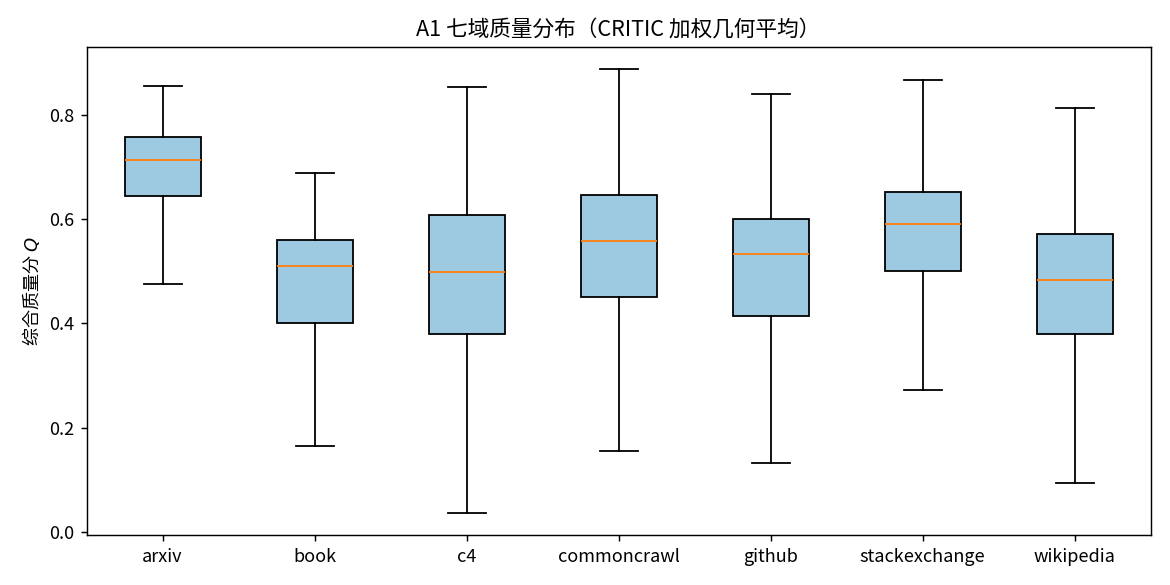
\includegraphics[width=.72\textwidth]{F2_domain_quality_box.png}
\caption{A1 七域质量分布（CRITIC 加权几何平均）。arxiv 显著最高；book 域仅 171 篇，其区间最宽。}
\label{fig:box}
\end{figure}

\subsection{问题一 (b)：指标冲突的定义、成因与消解}\label{sec:m1b}

\textbf{冲突定义（拒绝预设阈值）}。25 指标按信号来源分四组（规则型/DSIR/轻量分类器/模型评分器），组内 Kendall $W$ 分别为 $0.128/0.998/0.627/0.447$——同源信号一致性高，冲突主要发生在跨组，故在组级定义冲突：组分数取组内指标中位数，再转域内分位排名 $R_g(x)\in[0,1]$，冲突度 $c(x)=\max_g R_g-\min_g R_g$。阈值 $\tau$ 由冲突率—阈值曲线的最大曲率点确定（图~\ref{fig:conf}），得 $\tau=0.75$。

\textbf{测得冲突率 $21.5\%$}，直接否定《数据说明》页眉"冲突率约 $0\%$"的说法——后者以预设小阈值定义冲突再宣布无冲突，属把结论藏进定义。冲突与域强相关（$\chi^2=142.4$，$\mathrm{df}=6$，$p\approx10^{-23}$）；主冲突类型为"DSIR 高 $\times$ 规则型低"，在 A1/A2/A3 中占比 $19.6\%/15.1\%/18.1\%$，跨集复现；扩展集冲突率 $21.1\%$（A2）与 $22.9\%$（A3），与抽样集一致。对 30 篇高冲突文档的原文抽查（A1 含 \texttt{content}）证实两类机制：LaTeX/代码文本的专业价值高而表层流畅度指标低；模板化网页的规则统计量佳而模型评分器判为低教育价值。

\textbf{消解：Huber 连续降权}。对文档 $x$ 的组 $g$，按其排名偏离文档自身中位排名的程度 $\mathrm{dev}_g$ 施加权重 $u_g=\min(1,\tau_z/|\mathrm{dev}_g|)$，与 CRITIC 权重逐指标相乘后重归一，重算式~\eqref{eq:critic} 得修正分 $\widetilde Q$。效果：保序（$\rho(Q,\widetilde Q)=0.997$），冲突样本平均下调 $0.0033$ 而非冲突样本几乎不动（$-0.0004$）——降权而非删除，保留矛盾信息且不误伤专业语料；这是相对工业界硬过滤的改进点。严格口径的对照（冲突文档组分数取调和平均，下调 $0.149$）供敏感性使用。

\begin{figure}[H]
\centering
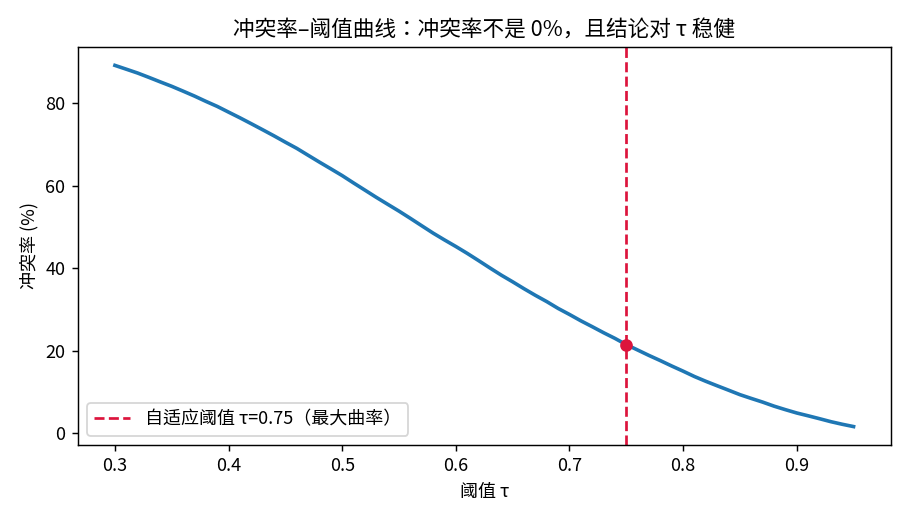
\includegraphics[width=.6\textwidth]{F3_conflict_rate_curve.png}
\caption{冲突率—阈值曲线与最大曲率点。结论在 $\tau\in[0.6,0.85]$ 内定性不变。}
\label{fig:conf}
\end{figure}

\subsection{跨体系桥接：17 个配比域的质量分}\label{sec:m1bridge}

11 个 inferred 域无官方质量信号。利用规则统计量\emph{可精确复算}的性质补全：自实现 11 个 \texttt{rps} 规则算子 $\Phi(\text{text})$，在 A1 上（每篇同时具备 $\Phi$ 与 $\widetilde Q$，$n=21{,}590$）以域分层五折交叉验证训练校准函数 $\hat g:\Phi\mapsto\widetilde Q$（梯度提升，$R^2_{\mathrm{cv}}=0.31$，优于岭回归 $0.25$）；再对 A18 的 17 域原文（31{,}340 篇）计算 $\hat Q=\hat g(\Phi)$ 并域级聚合。6 个有映射域上校准分与官方分互验：Pearson $0.70$、MAE $0.055$。最终 $\hat Q_d$ 取"映射域用官方分、inferred 域用校准分"，全部带 bootstrap CI 与证据等级标注（图~\ref{fig:bridge}）：最高 arxiv $0.716$，最低 dm\_mathematics $0.355$；ubuntu\_irc（16 篇）与 philpapers（63 篇）标注低置信。

\begin{figure}[H]
\centering
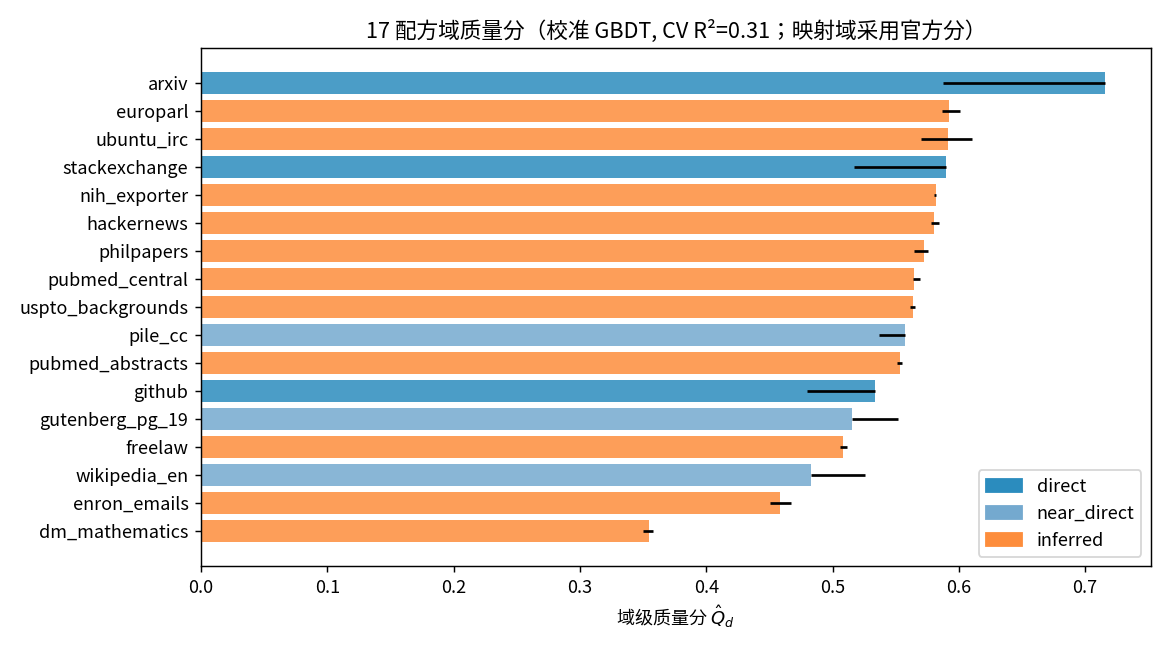
\includegraphics[width=.8\textwidth]{F4_bridge_17domains.png}
\caption{17 配比域质量分（颜色为映射类型；误差条为 bootstrap 95\% CI）。}
\label{fig:bridge}
\end{figure}

\subsection{问题一 (c)：配比—损失建模与最优配比}\label{sec:m1c}

\textbf{clr 变换消闭合效应（改进点）}。配比是成分数据：某域份额上升必然伴随其余域合计下降，直接回归会把机械的"此消彼长"误读为领域替代关系（Aitchison, 1986）。对 $\bm p$ 做中心对数比变换 $z_i=\ln(p_i/g(\bm p))$（$g$ 为几何均值，零分量乘性替换 $10^{-4}$），对每个验证域在对数空间回归：
\begin{equation}
\ln L_v=b_v+\sum_{i=1}^{17}\beta_{v,i}\,z_i+\varepsilon_v,
\qquad v=1,\dots,13,
\label{eq:clr}
\end{equation}
以 Huber 损失抗异常配方。1M 检验集（256 组）对照：\textbf{clr+Huber 的平均 $R^2=0.772$，裸配比 OLS（RegMix 原式）仅 $0.654$}（RMSE $0.320$ vs $0.432$）——闭合效应处理的收益即本方案对文献的量化改进。梯度提升作非线性对照（$R^2=0.897$），表明存在域间交互；故\emph{系数解释用线性、最优搜索用非线性}，两者在 $10^5$ 个候选配比上的目标损失秩相关 $0.77$，互为校验。

\textbf{迁移矩阵}。式~\eqref{eq:clr} 系数经链式法则折算到单纯形切空间，得 $T_{iv}=\partial\ln L_v/\partial p_i$（均匀配比处，图~\ref{fig:tm}）。全部 13 个自域效应为负（增配本域降本域损失），dm\_mathematics 自域效应最强（$-2.47$）；跨域外溢揭示 stackexchange 与 github 的互补结构。四个无损失列的域（nih\_exporter 等）保留为解释变量，其效应经由相对配比间接体现。

\begin{figure}[H]
\centering
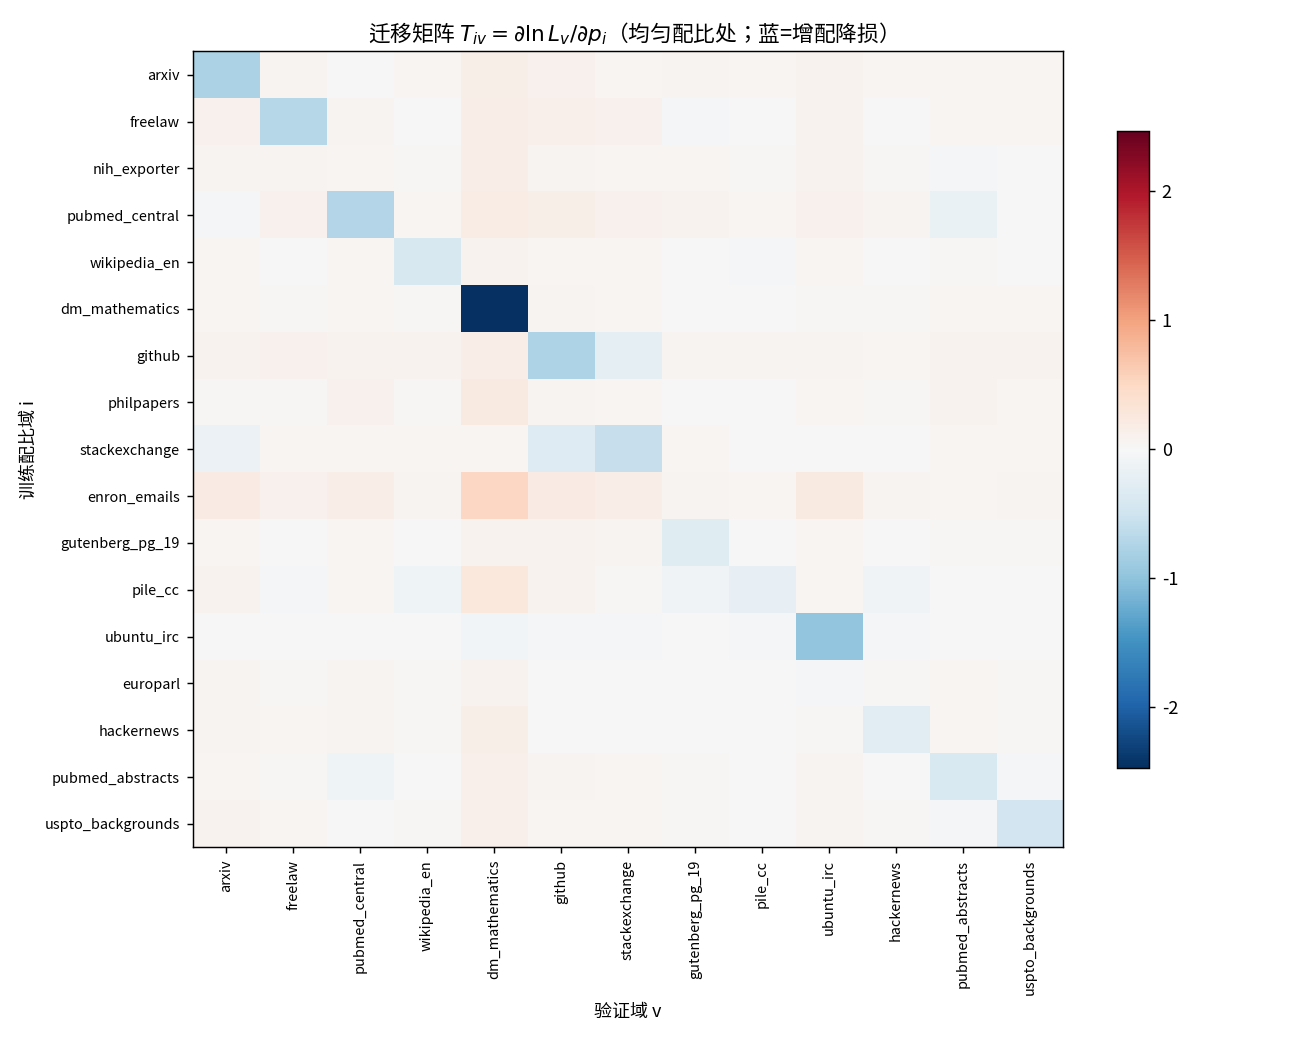
\includegraphics[width=.8\textwidth]{F5_transfer_matrix.png}
\caption{迁移矩阵 $T_{iv}$：蓝色为增配降损。对角占优，含非对角互补结构。}
\label{fig:tm}
\end{figure}

\textbf{质量交互项检验}。在式~\eqref{eq:clr} 加入 $\lambda_v\sum_ip_i(1-\hat Q_{d(i)})$ 作嵌套检验：$10/13$ 个验证域 $\lambda_v$ 显著（bootstrap 95\% CI 不含零）且加项后检验集 RMSE 全部不升；但\textbf{符号域间不一致}（中位数 $-0.249$，arxiv 域 $+0.79$）。结论：质量对配比—损失关系有独立解释力，但作用方向依验证域条件化——这提示问题二不应把质量与配比合并为单一乘子，二者应分开进入广义律。

\textbf{最优配比}。以训练配比均值为中心的多浓度 Dirichlet 采样 $10^5$ 个候选，取预测目标损失最优的前 100 个平均：等权口径 $\bm p^*$ 前五位为 pile\_cc $15.6\%$、stackexchange $10.0\%$、wikipedia $9.5\%$、pubmed\_central $9.1\%$、arxiv $8.9\%$；相对均匀配比预测降损 $9.9\%$（固定 $\bm p^*$ 的 bootstrap 95\% CI $[9.7\%,14.1\%]$）。pile\_cc 单域口径下 pile\_cc 占 $33.2\%$，复现 RegMix"网页语料对下游最有利"的反直觉结论。

\textbf{跨尺度验证与外推（假设~\ref{asm:proxy} 的检验）}。1M 系数直接预测三尺度留出集的目标损失排名：Spearman $0.52$（1M 留出）$/0.47$（60M）$/0.68$（1B）——排序中等保持；但 60M/1B 的绝对预测完全失效（$R^2$ 为大负值），系数漂移分解显示\textbf{截距显著下漂而斜率几乎不漂}（$\max_i|\rho_{\beta}|\approx0.007$）：配比效应结构稳定，基线水平随规模下移。对 A12--A15（10B/70B，幂律外推生成、非观测）：直接套 1M 系数 MAE $\approx3.5$ 完全不可用，以三尺度估计的漂移律 $b_v(N)=b_v^0+\rho_v\ln(N/10^6)$ 修正后 MAE 收窄至 $0.10$（35 倍改善）。外推稳健域排序：arxiv/pubmed\_central 最稳（$\rho>0.85$），pile\_cc/pubmed\_abstracts 最不稳（$\rho<0.40$）。

\textbf{质量 $\ne$ 训练价值}。域级质量分 $\hat Q_d$ 与训练边际价值 $\nu_d=-(\bar\beta_d-\overline{\bar\beta})$ 的秩相关 $\rho_{Q\nu}=-0.06$（图~\ref{fig:qv}）：内在质量几乎不预测训练价值，配比必须由实验回归而非质量排名确定。该结论直接支撑问题二将 $Q$ 与 $\bm p$ 设为两个独立自变量。

\begin{figure}[H]
\centering
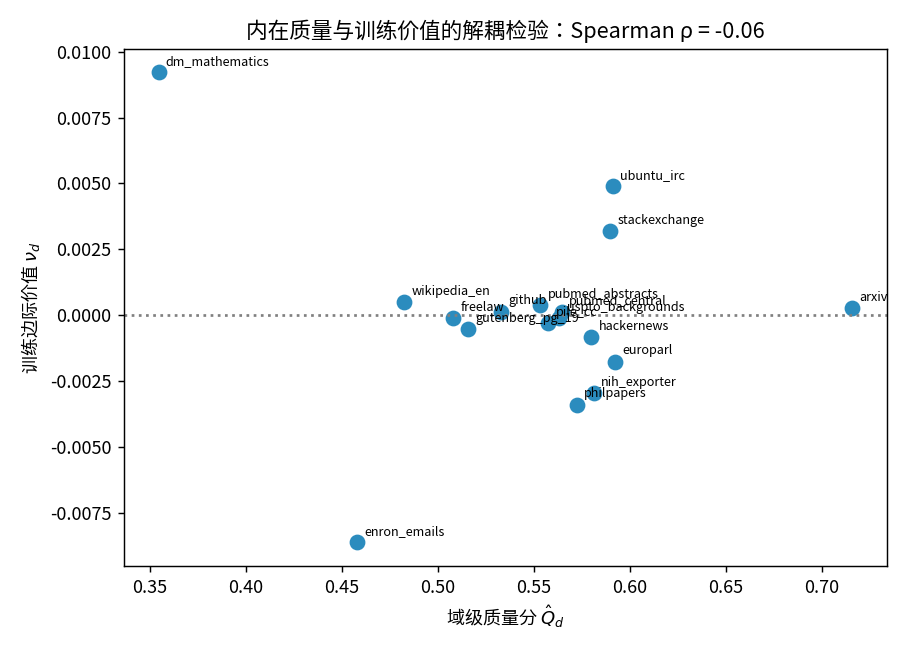
\includegraphics[width=.62\textwidth]{F7_quality_vs_value.png}
\caption{质量—价值解耦：dm\_mathematics 质量最低却训练边际价值最高。}
\label{fig:qv}
\end{figure}

\subsection{问题二：广义标度律的形式选择与拟合}\label{sec:m2fit}

\textbf{两步拟合}。第一步在 B1 上网格搜索 $(\alpha,\beta)$ 并最小二乘定 $(E,A,B)$，得 $L_0=1.6901+406.4N^{-0.340}+410.6D^{-0.280}$（$\mathrm{RMSE}=1.5\times10^{-4}$；该表呈公式生成特征，故此步为无噪声锚定）。第二步固定基线，在 B7（450 点）上对嵌套族做五折交叉验证：

\begin{table}[H]
\centering\small
\caption{质量项形式选择（cv-RMSE；数据噪声水平 $\sigma\approx0.05$）}
\begin{tabular}{lcc}
\toprule
候选形式 & cv-RMSE & 备注 \\
\midrule
耦合 + 地板（主） $\;h_N,h_D,k_0$ & $\bm{0.0497}$ & \textbf{主模型}（达噪声下限） \\
旧加性 $\;(1-Q)(k_0+k_1N^{-\alpha})$ & $0.0512$ & $\kappa_D=0$ 特例 \\
有效数据 $\;\kappa_N=0$ & $0.0979$ & 文献口径，单参数中最差 \\
\bottomrule
\end{tabular}
\label{tab:forms}
\end{table}

文献偏好的"质量折算有效数据量"乘子族（Muennighoff 风格）在本题数据上系统性落败——\emph{模型形式由交叉验证裁决而非先验借用}。主模型为

\begin{equation}
\boxed{\;L=\bigl\{E+A N^{-\alpha}h_N(Q)+B D^{-\beta}h_D(Q)+k_0(1-Q)\bigr\}\,e^{s(N)[\bar f(\bm p)-\bar f(\bm p^*)]}\;}
\label{eq:main}
\end{equation}

\begin{table}[H]
\centering\small
\caption{广义标度律参数（残差 bootstrap $B=300$）}
\begin{tabular}{cccccccc}
\toprule
$E$ & $A$ & $\alpha$ & $B$ & $\beta$ & $\kappa_N$ & $\kappa_D$ & $k_0$ \\
\midrule
$1.6901$ & $406.4$ & $0.340$ & $410.6$ & $0.280$ &
$\underset{[0.390,\,0.473]}{0.431}$ & $\underset{[0.085,\,0.195]}{0.140}$ &
$\underset{[0.114,\,0.168]}{0.141}$ \\
\bottomrule
\end{tabular}
\label{tab:params}
\end{table}

其中 $h_N=1+\kappa_N(1-Q)$，$h_D=1+\kappa_D(1-Q)$，$s(N)=\max\{1.003-0.077\log_{10}(N/10^6),0\}$。$Q=1$ 且 $\bm p=\bm p^*$ 时式~\eqref{eq:main} 退化为经典 Chinchilla 形式。主口径 $Q_{\mathrm B}=\bar q(\bm p)$，$Q_0=0.6609$。配比经问题一接口引入，不重复读取附件 A；域结构效应由迁移矩阵 $T$ 单独描述。

\textbf{跨源检验}。真实文献点上主模型预测与观测的 Spearman：scaling\_baseline（57 点）$0.983$、published（44 点）$0.959$，平均偏差 $0.22/0.02$ nats——趋势一致，绝对偏移源于 tokenizer 与验证集差异，符合"跨源只比趋势"的审计原则；B2（Cerebras 半合成）偏差 $1.18$ nats，仅作定性佐证。

\subsection{问题二：解析理论}\label{sec:m2theory}

以下命题由式~\eqref{eq:main} 直接推导，全部与数值优化互验（相对误差 $<10^{-6}$）。

\begin{proposition}[弹性]\label{prop:el}
记 $\Phi=\kappa_N AN^{-\alpha}+\kappa_D BD^{-\beta}+k_0$，则
$\displaystyle
\varepsilon_N=-\frac{\alpha A N^{-\alpha}h_N}{L},\quad
\varepsilon_D=-\frac{\beta B D^{-\beta}h_D}{L},\quad
\varepsilon_Q=-\frac{Q\,\Phi}{L}.$
在 $(N,D,Q)=(10^{10},10^{12},0.9)$ 处三者为 $-0.028/-0.025/-0.103$：\emph{质量弹性约为参数弹性的 $3.7$ 倍}。
\end{proposition}

\begin{proposition}[质量—参数等效替代及其边界]\label{prop:sub}
固定 $D$，使 $L(N',D,Q)=L(N,D,Q+\delta)$ 的等效参数量
\begin{equation}
\frac{N'}{N}=t^{-1/\alpha},\quad
t=\frac{h_N(Q+\delta)}{h_N(Q)}-\frac{\delta(\kappa_D BD^{-\beta}+k_0)}{AN^{-\alpha}h_N(Q)},
\end{equation}
当且仅当 $t>0$ 时有限。算力最优点上 $Q_{\mathrm B}:0.5\to0.6$ 等效参数 $1.29/1.42/1.77$ 倍（$C=10^{20}/10^{22}/10^{24}$）。同一份质量改进，模型越大越值钱。
\end{proposition}

\begin{proposition}[质量地板]\label{prop:fl}
$\lim_{N,D\to\infty}L=E+(1-Q)k_0$。$Q=0.5$ 的地板比 $Q=1$ 高 $0.070$ nats。该地板是 B6/B7 的生成特征，外推须标注。
\end{proposition}

\begin{proposition}[算力最优配置随质量移动]\label{prop:opt}
约束 $6ND=C$ 下，
\begin{equation}
N^{*}(C,Q)=\Bigl[\frac{\alpha A\,h_N(Q)}{\beta B\,h_D(Q)}\Bigr]^{\frac{1}{\alpha+\beta}}
\Bigl(\frac{C}{6}\Bigr)^{\frac{\beta}{\alpha+\beta}},\qquad \frac{\beta}{\alpha+\beta}=0.452.
\end{equation}
因为 $\kappa_N>\kappa_D$，质量越低最优模型越大：$Q_{\mathrm B}=0.3$ 时的 $N^*$ 是 $Q_{\mathrm B}=1$ 时的 $1.32$ 倍。$C=10^{22}$ 时最优 token/参数比从 $Q=0.3$ 的 36 升至 $Q=1$ 的 63。
\end{proposition}

\begin{figure}[H]
\centering
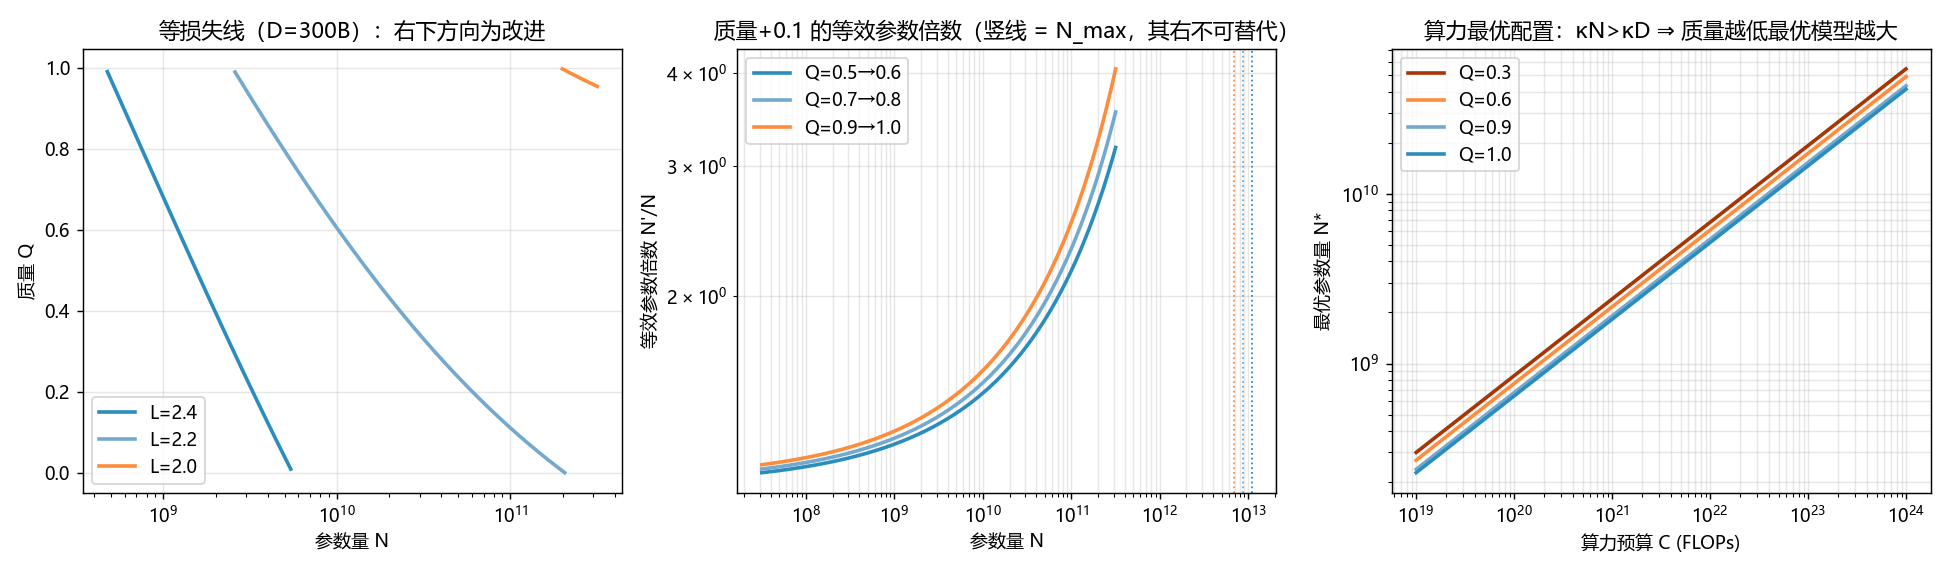
\includegraphics[width=\textwidth]{F21_theory.png}
\caption{解析理论三联图：等损失线（左）、等效参数倍数（中）、$N^*(C,Q)$（右）。}
\label{fig:theory}
\end{figure}

\section{模型检验}

\subsection{检验体系总览}

\begin{table}[H]
\centering\small
\caption{检验清单：方法关系、判据与结果}
\begin{tabular}{p{3.6cm}p{2.1cm}p{3.4cm}p{4.6cm}}
\toprule
检验对 & 关系类型 & 判据 & 结果 \\
\midrule
CRITIC vs PCA/TOPSIS/等权 & 互相验证 & 样本级 Spearman & $0.871/0.946/0.991$，排序稳健 \\
clr 线性 vs 梯度提升 & 互相验证 & $10^5$ 采样点秩相关 & $0.77$，$\bm p^*$ 非模型形式幻觉 \\
clr vs 裸 OLS & 改进证据 & 检验集 $R^2$/RMSE & $0.772$ vs $0.654$，闭合效应实证 \\
A1 vs A2/A3 全量 & 代表性检验 & KS、Cohen's $d$ & $p=0.60/0.12$，$d\approx0.005$ \\
冲突结论跨集复现 & 稳健性 & 冲突率与主类型 & $21.5\%/21.1\%/22.9\%$，类型一致 \\
1M$\to$60M$\to$1B & 假设~\ref{asm:proxy} 检验 & 排名 Spearman & $0.52/0.47/0.68$；截距漂、斜率稳 \\
10B/70B 外推表 & 稳健性讨论 & 修正前后 MAE & $3.5\to0.10$（非观测，只作讨论） \\
线性乘性耦合 vs 有效数据 & 形式选择 & 五折 cv-RMSE & $0.0497$ vs $0.0979$ \\
解析解 vs 数值优化 & 互相验证 & 相对误差 & $<10^{-6}$（命题 2、4） \\
标度律 vs 真实文献点 & 外部合理性 & 趋势 Spearman & $0.959$--$0.983$，仅比趋势 \\
质量分 vs 训练价值 & 概念区分 & $\rho_{Q\nu}$ & $-0.06$：分歧本身即结论 \\
\bottomrule
\end{tabular}
\label{tab:checks}
\end{table}

三点说明。其一，"互相验证"仅用于\emph{同一问题、不同假设}的方法对（如 CRITIC 与 PCA），判据取排序一致性；分工衔接的上下游方法（如冲突分析与配比回归）之间不存在验证关系，不作此类声称。其二，不一致处同样是结论：$\rho_{Q\nu}=-0.06$ 是"内在质量 $\ne$ 训练价值"的定量证据而非检验失败；60M/1B 的绝对预测失效（$R^2$ 大负值）源于截距漂移，恰好论证了"跨尺度外推必须做尺度修正"并给出修正后 35 倍的误差收窄。其三，A12--A15 与 B8 的证据等级（外推生成/不同源）全程继承标注，未升格为实证。

\subsection{灵敏度分析}

\textbf{冲突阈值}：$\tau\in[0.6,0.85]$ 内冲突率 $12\%$--$35\%$ 连续变化，域排序与主冲突类型不变。\textbf{评价权重}：等权与 pile\_cc 单域两口径下 $\bm p^*$ 的头部域一致（pile\_cc 居首），仅集中度不同。\textbf{质量口径锚点}（假设~\ref{asm:anchor}）：主口径 $Q_0=0.6609$ 与副口径 $Q_{\mathrm B}=\bar q/0.6609$ 下，$Q_{\mathrm B}:0.5\to0.6$ 的等效倍数为 $1.29/1.42/1.77$ 与 $1.47/1.73/2.48$（$C=10^{20}/10^{22}/10^{24}$），方向不变。\textbf{消解规则}：Huber 降权与调和平均两口径下域级质量排序 Spearman $>0.95$。\textbf{bootstrap}：$\kappa_N,\kappa_D,k_0$ 的 95\% CI 为 $[0.390,0.473]$、$[0.085,0.195]$、$[0.114,0.168]$，$P(\kappa_N>\kappa_D)=1$。

\section{模型的优缺点与改进方向}

\textbf{优点}：(i) 全流程证据分层，半合成与外推数据未混入主结论；(ii) 冲突率、闭合效应、质量—价值解耦三处以量化证据修正了《数据说明》页眉与文献的现成说法；(iii) 广义标度律的形式由交叉验证从五种候选中裁决，且四条解析命题全部闭式可验；(iv) 问题一至问题二的接口（$Q$ 口径、$\bm p^*$、迁移矩阵、漂移律）落盘为文件，问题三、四可直接消费。

\textbf{缺点与改进}：(i) 17 域质量分中 11 个 inferred 域依赖校准函数（$R^2_{\mathrm{cv}}=0.31$），信息量有限，若增补这些域的模型评分器信号可显著收紧区间；(ii) 质量交互项 $\lambda$ 符号域间不一致的机制尚未解释，需按验证域类型分层建模；(iii) B 附件为半合成数据，$\kappa_N,\kappa_D,k_0$ 的绝对数值不宜直接外推到真实训练体系；(iv) $s(N)$ 只在 1M--1B 上标定，1B 以上是外推。

\section{结论}

问题一建立了从 22 个异质信号到连续质量分的可复现管线，测得并消解了 $21.5\%$ 的指标冲突，以 clr 回归给出 17 域配比的迁移矩阵与最优配比（预测降损 $9.9\%$），并发现内在质量与训练价值近乎正交。问题二以数据裁决的线性乘性耦合建立广义标度律，主口径 $Q_0=0.6609$。四条解析推论——质量弹性约为参数弹性的 $3.7$ 倍、等效替代随规模从 $1.29$ 倍放大到 $1.77$ 倍、质量地板的存在、最优配置随质量向"小模型多数据"移动——共同刻画了"数据质量是与算力并列的一等资源"这一核心判断。

\begin{table}[H]
\centering\small
\caption{问题一、二产出与下游接口}
\begin{tabular}{lll}
\toprule
产出 & 内容 & 下游用途 \\
\midrule
P1-Q\_sample / Q\_domain & 27.2 万样本级 $Q$；17 域 $\hat Q_d$ 及 CI & 问题二 $\bar Q(\bm p)$；问题三 $Q_0$ \\
P1-$f(\bm p)$ / $T$ & 配比回归系数；$17\times13$ 迁移矩阵 & 问题三损失项；领域互补分析 \\
P1-$\bm p^*$ & 双口径最优配比，$\bar Q(\bm p^*)$ & 问题三默认配比 \\
P1-rank\_decay & 排名保持度随 $N$ 的三点曲线 & 外推不确定性口径 \\
P2-params / theory & 式~\eqref{eq:main} 全参数与 CI；$N^*(C,Q)$ 闭式 & 问题三目标函数与优化初值 \\
\bottomrule
\end{tabular}
\label{tab:iface}
\end{table}

\begin{thebibliography}{9}\small
\bibitem{hoffmann} Hoffmann J, et al. Training Compute-Optimal Large Language Models. NeurIPS 2022.
\bibitem{regmix} Liu Q, et al. RegMix: Data Mixture as Regression for Language Model Pre-training. ICLR 2025.
\bibitem{metarater} SlimPajama-Meta-rater 数据集（OpenDataLab）：多维质量信号体系.
\bibitem{fineweb} Penedo G, et al. The FineWeb Datasets. NeurIPS 2024（FineWeb-Edu 教育价值过滤）.
\bibitem{muennighoff} Muennighoff N, et al. Scaling Data-Constrained Language Models. NeurIPS 2023.
\bibitem{aitchison} Aitchison J. The Statistical Analysis of Compositional Data. Chapman \& Hall, 1986.
\bibitem{critic} Diakoulaki D, Mavrotas G, Papayannakis L. Determining objective weights in multiple criteria problems: The CRITIC method. Computers \& Operations Research, 1995.
\bibitem{huber} Huber P J. Robust estimation of a location parameter. Ann. Math. Statist., 1964.
\bibitem{pythia} Biderman S, et al. Pythia: A Suite for Analyzing Large Language Models. ICML 2023.
\end{thebibliography}

\appendix
\section*{附录：AI 使用披露}
依据赛题规定，AI 工具仅用于资料整理、代码调试与文字排版辅助；本文的模型选择、公式推导、结果分析与论证由参赛队完成并逐项复核。全部数值结果可由随文代码（\texttt{code\_q1/}、\texttt{code\_q2/}）在附件数据上复现。


\end{document}
